\chapter{Experiments}

% feedback Benjamin
% Structuur sectie
% Eerst in kleine sectie experimenten oplijsten
% Subsecties
% - Experiment 1
% - Experiment 2
% Experimenten is ruimte om resultaten te schrijven
% Eerste observaties

% Explain first which experiments are done and why
% Per section: - Write down results of experiments

\section{Localization evaluation}
We evaluate the five \acrshort{wsol} methods that are described in detail in section \ref{lb:wsol_methods}: CAM, Grad-CAM, Grad-CAM++, Score-CAM and MinMaxCAM. All these methods, except Grad-CAM, are evaluated using a VGG-GAP network and a ResNet-50 network. Grad-CAM is a generalization of CAM that yields the same score maps as CAM in a \acrshort{cnn} with a \acrshort{gap} layer like the VGG16-GAP and ResNet-50 networks. Grad-CAM, Grad-CAM++ and Score-CAM are also evaluated using a VGG16 network. As these methods don't require an architecture with \acrshort{gap} layer, it is interesting to see how they perform on the unmodified VGG16 architecture.

The localization methods are evaluated for the mentioned networks on the synthetic datasets and on the ImageNet dataset. For the VGG16-GAP network and the ResNet-50 network, we trained two models per network on the synthetic datasets: One without regularization and one with MinMaxCAM regularization. CAM, Grad-CAM++ and Score-CAM are evaluated on the models trained without regularization and MinMaxCAM on the models with regularization. For the VGG16 network we only train one model without regularization per synthetic dataset as MinMaxCAM is not compatible with this network. Evaluation on the ImageNet dataset is done for pre-trained networks, except for MinMaxCAM which requires training due to its regularization stage.

\subsection{Synthetic dataset}
We evaluate the \acrshort{cam} methods on the synthetic datasets listed in Table \ref{tab:synthetic_datasets}, using the MaxBoxAccV3 and PxAP metrics. In following sections, results for VGG16-GAP, VGG16 and ResNet-50 architectures are discussed.

\subsubsection{VGG16-GAP}
The localization results using the multiple-instance \acrshort{wsol} metric MaxBoxAccV3 recall and precision are shown in Table \ref{tab:maxboxaccv3_recall_vgg16_gap_synthetic} and Table \ref{tab:maxboxaccv3_precision_vgg16_gap_synthetic}. The pixel average precision results are illustrated in Table \ref{tab:pxap_vgg16_gap_synthetic}. In each table the column-wise maximum value per dataset is highlighted in green and the column-wise minimum per dataset is marked in red. From the results, some interesting observations can be noticed.
\begin{table}[ht]
\centering
\begin{tabular}{lrrrrrrrr}
\toprule
 & \multicolumn{8}{c}{VGG16-GAP synthetic (MaxBoxAccV3 recall)} \\
method & d1b & d1t & d2b & d2t & d3b & d3t & d4b & d4t \\
\cmidrule(lr){1-1} \cmidrule(lr){2-9} 
CAM & \color{purple} \bfseries 93.67 & 91.67 & \color{purple} \bfseries 66.58 & 65.67 & \color{purple} \bfseries 60.94 & 59.11 & 48.67 & 54.87 \\
Grad-CAM++ & 94.17 & \color{teal} \bfseries 92.50 & 67.33 & \color{purple} \bfseries 65.08 & 62.50 & 59.11 & \color{purple} \bfseries 48.42 & 55.17 \\
MinMaxCAM & \color{teal} \bfseries 94.83 & 89.33 & 67.33 & 65.17 & 62.83 & \color{purple} \bfseries 57.67 & 48.87 & \color{purple} \bfseries 43.33 \\
Score-CAM & 94.17 & \color{purple} \bfseries 88.83 & \color{teal} \bfseries 73.00 & \color{teal} \bfseries 68.08 & \color{teal} \bfseries 69.33 & \color{teal} \bfseries 65.11 & \color{teal} \bfseries 51.37 & \color{teal} \bfseries 56.58 \\
\bottomrule
\end{tabular}
\caption[MaxBoxAccV3 for VGG16-GAP on synthetic datasets]{MaxBoxAccV3 recall for VGG16-GAP on synthetic datasets.}
\label{tab:maxboxaccv3_recall_vgg16_gap_synthetic}
\end{table}

\begin{table}[ht]
\centering
\begin{tabular}{lrrrrrrrr}
\toprule
 & \multicolumn{8}{c}{VGG16-GAP synthetic (MaxBoxAccV3 precision)} \\
method & d1b & d1t & d2b & d2t & d3b & d3t & d4b & d4t \\
\cmidrule(lr){1-1} \cmidrule(lr){2-9} 
CAM & 88.57 & 84.86 & 73.39 & 71.86 & \color{purple} \bfseries 69.34 & 65.39 & 63.22 & 63.96 \\
Grad-CAM++ & 88.82 & \color{teal} \bfseries 86.57 & \color{purple} \bfseries 72.96 & 71.42 & 69.63 & 64.82 & \color{purple} \bfseries 62.94 & 63.56 \\
MinMaxCAM & \color{teal} \bfseries 89.09 & 83.47 & 73.50 & \color{teal} \bfseries 72.66 & 71.91 & \color{purple} \bfseries 63.68 & 63.46 & \color{purple} \bfseries 52.37 \\
Score-CAM & \color{purple} \bfseries 87.51 & \color{purple} \bfseries 78.66 & \color{teal} \bfseries 76.77 & \color{purple} \bfseries 71.35 & \color{teal} \bfseries 74.79 & \color{teal} \bfseries 69.70 & \color{teal} \bfseries 64.36 & \color{teal} \bfseries 63.96 \\
\bottomrule
\end{tabular}
\caption[MaxBoxAccV3 for VGG16-GAP on synthetic datasets]{MaxBoxAccV3 precision for VGG16-GAP on synthetic datasets.}
\label{tab:maxboxaccv3_precision_vgg16_gap_synthetic}
\end{table}

\begin{table}[ht]
\centering
\begin{tabular}{lrrrrrrrr}
\toprule
 & \multicolumn{8}{c}{VGG16-GAP synthetic (PxAP)} \\
method & d1b & d1t & d2b & d2t & d3b & d3t & d4b & d4t \\
\cmidrule(lr){1-1} \cmidrule(lr){2-9} 
CAM & 80.82 & \color{purple} \bfseries 80.45 & 78.52 & 74.68 & 76.31 & 72.79 & \color{purple} \bfseries 65.69 & 72.55 \\
Grad-CAM++ & \color{teal} \bfseries 81.82 & \color{teal} \bfseries 81.56 & \color{teal} \bfseries 79.33 & \color{teal} \bfseries 74.96 & \color{teal} \bfseries 77.90 & 73.20 & 66.92 & 73.21 \\
MinMaxCAM & 81.29 & 80.46 & 78.62 & \color{purple} \bfseries 74.00 & \color{purple} \bfseries 75.44 & \color{purple} \bfseries 71.43 & 66.10 & \color{purple} \bfseries 57.24 \\
Score-CAM & \color{purple} \bfseries 80.71 & 81.07 & \color{purple} \bfseries 77.96 & 74.32 & 77.64 & \color{teal} \bfseries 75.10 & \color{teal} \bfseries 67.34 & \color{teal} \bfseries 73.45 \\
\bottomrule
\end{tabular}
\caption[PxAP for VGG16-GAP on synthetic datasets]{PxAP for VGG16-GAP on synthetic datasets.}
\label{tab:pxap_vgg16_gap_synthetic}
\end{table}

\textbf{Multi-instance localization recall and precision} drop for datasets with increasing number of object instances. MaxBoxAccV3 recall is above or close to 90\% for the single instance datasets d1b and d1t. The localization performance for the 2-instance and 3-instance datasets is =significantly lower than the performance for the single instance datasets. Localization performance is worst for the dataset with four instances per image, although still about half of all object instances can be localized with a model that is trained for classification only.

\textbf{Pixel average precision} doesn't drop as significantly as the MaxBoxAccV3 metrics for images with multiple object instances. Intuitively, a reasonable explanation is a mismatch at pixel-level causes a less severe penalty than a mismatch at the coarse-grained bounding box level.

\textbf{Best MaxBoxAccV3 recall for multiple instances} is obtained by Score-CAM. The promising results for multi-target visualization observed by Wang \textit{et al.} \cite{wang2020score}, seem to hold in our quantitative evaluation. 

\textbf{Discrepancy between datasets having images with (b variant) and without background (t variant)}. When we pairwise compare datasets with the same number of object instances, we see that for nearly all cases, experiments with datasets having images with background (variant b) show better MaxBoxAccV3 precision and recall than dataset variants without background images. The datasets with four instances are the exception for CAM, Grad-CAM++ and Score-CAM. The results for these localization methods follow the same trend as they are evaluated on the same model trained without regularization. 

The discrepancies can be explained by comparing the training classification and localization accuracy. Fig. \ref{fig:loc_vs_acc_vgg16_gap_cam_synthetic}  illustrates these metrics for the VGG16-GAP network trained for CAM on the datasets. Pair-wise comparison of localization accuracy for datasets with same number of object instances, shows that images with background have higher accuracy, except for d4b and d4t. Here we can see that classification and localization accuracy for d4b show a drop at training epoch 15. Because we use an early training stop criterion that quits training after five epochs if the validation loss hasn't improved (i.e. lower than best loss so far), localization accuracy cannot further improve.

\begin{figure}[ht]
    \begin{center}       
    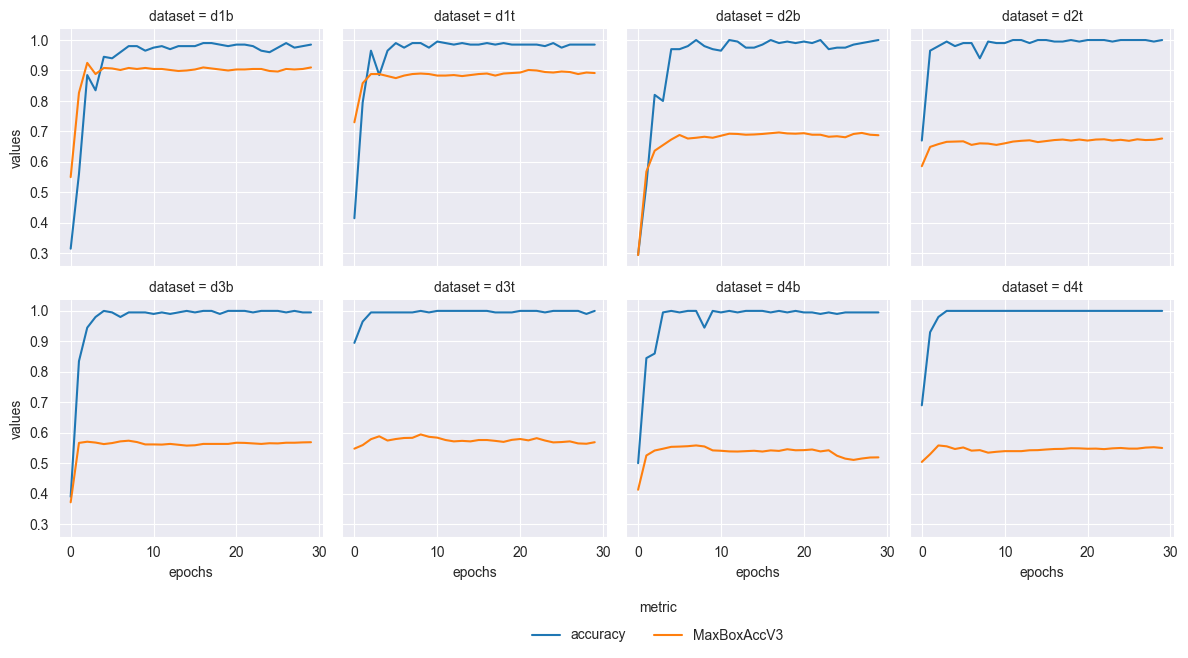
\includegraphics[width=\textwidth]{fig_loc_vs_acc_vgg16_gap_cam_synthetic.png}
    \caption[Training classification versus localization accuracy for CAM on VGG16-GAP]{Training classification versus localization accuracy (MaxBoxAccV3 recall) for CAM on VGG16-GAP.}
    \caption*{Source: Author}
    \label{fig:loc_vs_acc_vgg16_gap_cam_synthetic}
    \end{center}
\end{figure}

Figure \ref{fig:loc_vs_acc_vgg16_gap_minmaxcam_synthetic} shows training classification and localization accuracy for CAM models fine-tuned with MinMaxCAM regularization on the different datasets. This explains the rather flat training curves. While classification and localization accuracy for datasets having images with background (b variants) slightly increase, the metrics decrease for the datasets having images without background (t variants). This observation correlates with the metrics shown in Table \ref{tab:maxboxaccv3_recall_vgg16_gap_synthetic}. Wang \textit{et al.} \cite{wang2021minmaxcam} set out the condition for common region regularization to work, that a set of images for the same class should have different backgrounds. This clearly is not the case for the t-variant datasets. Intuitively, this explains the lower accuracy scores.

\begin{figure}[ht]
    \begin{center}       
    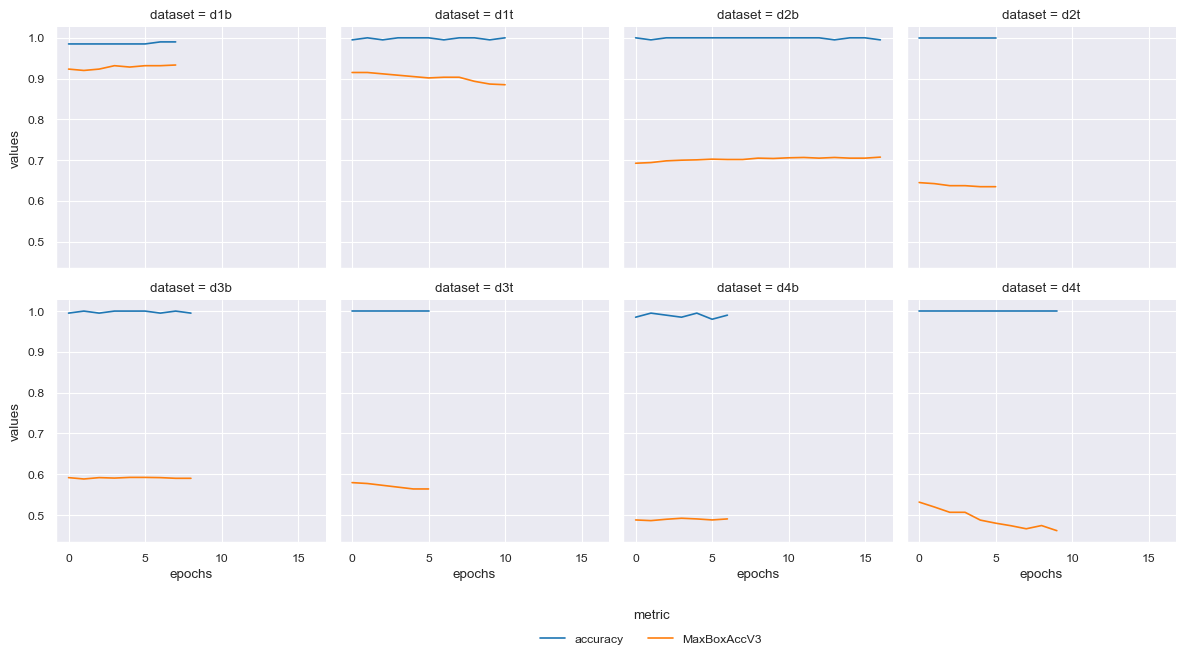
\includegraphics[width=\textwidth]{fig_loc_vs_acc_vgg16_gap_minmaxcam_synthetic.png}
    \caption[Training classification versus localization accuracy for MinMaxCAM on VGG16-GAP]{Training classification versus localization accuracy (MaxBoxAccV3 recall) for MinMaxCAM on VGG16-GAP.}
    \caption*{Source: Author}
    \label{fig:loc_vs_acc_vgg16_gap_minmaxcam_synthetic}
    \end{center}
\end{figure}

\subsubsection{VGG16}
The localization results for VGG16 on the synthetic datasets are shown in Table \ref{tab:maxboxaccv3_recall_vgg16_base_synthetic} for MaxBoxAccV3 recall, in Table \ref{tab:maxboxaccv3_precision_vgg16_base_synthetic} for MaxBoxAccV3 precision, and in Table \ref{tab:pxap_vgg16_base_synthetic} for the PxAP metric. Note that CAM and MinMaxCAM methods cannot be used on VGG16 as this architecture has no \acrshort{gap} layer. Grad-CAM is used here as generalization of CAM.

\begin{table}[ht]
\centering
\begin{tabular}{lrrrrrrrr}
\toprule
 & \multicolumn{8}{c}{VGG16 synthetic (MaxBoxAccV3 recall)} \\
method & d1b & d1t & d2b & d2t & d3b & d3t & d4b & d4t \\
\cmidrule(lr){1-1} \cmidrule(lr){2-9} 
Grad-CAM & \color{teal} \bfseries 82.83 & \color{teal} \bfseries 77.33 & \color{teal} \bfseries 56.08 & 37.33 & \color{teal} \bfseries 55.17 & 44.39 & 48.79 & 40.21 \\
Grad-CAM++ & \color{purple} \bfseries 77.00 & \color{purple} \bfseries 70.83 & \color{purple} \bfseries 40.92 & \color{purple} \bfseries 26.83 & \color{purple} \bfseries 47.39 & \color{purple} \bfseries 37.33 & \color{purple} \bfseries 40.17 & \color{purple} \bfseries 34.08 \\
Score-CAM & 81.83 & 74.50 & 55.00 & \color{teal} \bfseries 44.58 & 54.44 & \color{teal} \bfseries 48.56 & \color{teal} \bfseries 51.04 & \color{teal} \bfseries 45.79 \\
\bottomrule
\end{tabular}
\caption[MaxBoxAccV3 recall for VGG16 on synthetic datasets]{MaxBoxAccV3 recall for VGG16 on synthetic datasets.}
\label{tab:maxboxaccv3_recall_vgg16_base_synthetic}
\end{table}

\begin{table}[ht]
\centering
\begin{tabular}{lrrrrrrrr}
\toprule
 & \multicolumn{8}{c}{VGG16 synthetic (MaxBoxAccV3 precision)} \\
method & d1b & d1t & d2b & d2t & d3b & d3t & d4b & d4t \\
\cmidrule(lr){1-1} \cmidrule(lr){2-9}
Grad-CAM & 60.23 & 47.89 & \color{teal} \bfseries 57.65 & 39.36 & 57.08 & 42.90 & 51.59 & 46.86 \\
Grad-CAM++ & \color{purple} \bfseries 34.13 & \color{purple} \bfseries 31.95 & \color{purple} \bfseries 36.21 & \color{purple} \bfseries 21.59 & \color{purple} \bfseries 43.89 & \color{purple} \bfseries 29.09 & \color{purple} \bfseries 36.42 & \color{purple} \bfseries 30.13 \\
Score-CAM & \color{teal} \bfseries 66.28 & \color{teal} \bfseries 57.89 & 55.51 & \color{teal} \bfseries 47.12 & \color{teal} \bfseries 57.25 & \color{teal} \bfseries 50.51 & \color{teal} \bfseries 55.35 & \color{teal} \bfseries 52.23 \\
\bottomrule
\end{tabular}
\caption[MaxBoxAccV3 precision for VGG16 on synthetic datasets]{MaxBoxAccV3 precision for VGG16 on synthetic datasets.}
\label{tab:maxboxaccv3_precision_vgg16_base_synthetic}
\end{table}

\begin{table}[ht]
\centering
\begin{tabular}{lrrrrrrrr}
\toprule
 & \multicolumn{8}{c}{VGG16 synthetic (PxAP)} \\
method & d1b & d1t & d2b & d2t & d3b & d3t & d4b & d4t \\
\cmidrule(lr){1-1} \cmidrule(lr){2-9}
Grad-CAM & \color{teal} \bfseries 71.14 & \color{teal} \bfseries 65.89 & 60.66 & 42.86 & 61.69 & 46.63 & 56.26 & 50.54 \\
Grad-CAM++ & \color{purple} \bfseries 66.88 & \color{purple} \bfseries 59.54 & \color{purple} \bfseries 49.45 & \color{purple} \bfseries 29.74 & \color{purple} \bfseries 56.42 & \color{purple} \bfseries 40.43 & \color{purple} \bfseries 50.40 & \color{purple} \bfseries 39.47 \\
Score-CAM & 69.19 & 65.12 & \color{teal} \bfseries 61.79 & \color{teal} \bfseries 50.66 & \color{teal} \bfseries 62.64 & \color{teal} \bfseries 56.56 & \color{teal} \bfseries 58.82 & \color{teal} \bfseries 56.15 \\
\bottomrule
\end{tabular}
\caption[PxAP for VGG16 on synthetic datasets]{PxAP for VGG16 on synthetic datasets.}
\label{tab:pxap_vgg16_base_synthetic}
\end{table}

We see the same pair-wise discrepancies between datasets having the same object instances and different variant (with or without background image) as observed for the VGG16-GAP network. An additional observation is that the localization metrics for VGG16 are lower than those of the VGG16-GAP network on the same datasets. Intuitively, in the VGG16 network there is a less direct relationship between feature activation in the last convolutional layer and the predicted target due to the dense network between the convolutional backbone and the classification output. Another important observation is that Grad-CAM++ performs worst for all metrics.

\subsubsection{ResNet-50}
Localization performance results for the ResNet-50 network on the synthetic dataset are illustrated in Table \ref{tab:maxboxaccv3_recall_resnet50_synthetic} for MaxBoxAccV3 recall, in Table \ref{tab:maxboxaccv3_precision_resnet50_synthetic} for MaxBoxAccV3 precision and in Table \ref{tab:pxap_resnet50_synthetic} for PxAP. Here Grad-CAM is not evaluated as it performs the same as CAM for architectures with a \acrshort{gap} architecture.

\begin{table}[ht]
\centering
\begin{tabular}{lrrrrrrrr}
\toprule
 & \multicolumn{8}{c}{ResNet-50 synthetic (MaxBoxAccV3 recall)} \\
method & d1b & d1t & d2b & d2t & d3b & d3t & d4b & d4t \\
\cmidrule(lr){1-1} \cmidrule(lr){2-9}
CAM & 82.83 & 65.50 & 62.00 & 60.67 & 63.44 & 59.61 & 57.67 & 52.62 \\
Grad-CAM++ & \color{teal} \bfseries 83.83 & 67.67 & \color{teal} \bfseries 63.67 & 65.08 & 65.39 & 61.67 & \color{teal} \bfseries 60.79 & 53.58 \\
MinMaxCAM & \color{purple} \bfseries 75.33 & \color{purple} \bfseries 60.67 & \color{purple} \bfseries 57.58 & \color{purple} \bfseries 48.92 & \color{purple} \bfseries 52.00 & \color{purple} \bfseries 53.72 & \color{purple} \bfseries 54.33 & \color{purple} \bfseries 49.92 \\
Score-CAM & 80.50 & \color{teal} \bfseries 69.67 & 62.33 & \color{teal} \bfseries 66.25 & \color{teal} \bfseries 65.44 & \color{teal} \bfseries 63.44 & 58.83 & \color{teal} \bfseries 56.17 \\
\bottomrule
\end{tabular}
\caption[MaxBoxAccV3 recall for ResNet-50 on synthetic datasets]{MaxBoxAccV3 recall for ResNet-50 on synthetic datasets.}
\label{tab:maxboxaccv3_recall_resnet50_synthetic}
\end{table}

\begin{table}[ht]
\centering
\begin{tabular}{lrrrrrrrr}
\toprule
 & \multicolumn{8}{c}{ResNet-50 synthetic (MaxBoxAccV3 precision)} \\
method & d1b & d1t & d2b & d2t & d3b & d3t & d4b & d4t \\
\cmidrule(lr){1-1} \cmidrule(lr){2-9}
CAM & 74.27 & 52.56 & 64.18 & 64.47 & 68.11 & 63.30 & 63.84 & 58.63 \\
Grad-CAM++ & \color{teal} \bfseries 75.63 & 55.49 & \color{teal} \bfseries 64.77 & 68.09 & \color{teal} \bfseries 69.15 & 64.90 & \color{teal} \bfseries 65.79 & 58.81 \\
MinMaxCAM & \color{purple} \bfseries 64.47 & \color{purple} \bfseries 45.72 & \color{purple} \bfseries 60.08 & \color{purple} \bfseries 49.78 & \color{purple} \bfseries 57.44 & \color{purple} \bfseries 56.71 & \color{purple} \bfseries 61.95 & \color{purple} \bfseries 56.49 \\
Score-CAM & 73.90 & \color{teal} \bfseries 58.39 & 62.94 & \color{teal} \bfseries 68.44 & 68.17 & \color{teal} \bfseries 65.84 & 63.99 & \color{teal} \bfseries 61.00 \\
\bottomrule
\end{tabular}
\caption[MaxBoxAccV3 precision for ResNet-50 on synthetic datasets]{MaxBoxAccV3 precision for ResNet-50 on synthetic datasets.}
\label{tab:maxboxaccv3_precision_resnet50_synthetic}
\end{table}

\begin{table}[ht]
\centering
\begin{tabular}{lrrrrrrrr}
\toprule
 & \multicolumn{8}{c}{ResNet-50 synthetic (PxAP)} \\
method & d1b & d1t & d2b & d2t & d3b & d3t & d4b & d4t \\
\cmidrule(lr){1-1} \cmidrule(lr){2-9} 
CAM & 71.89 & 57.79 & 70.16 & 71.97 & 71.62 & 70.04 & 69.90 & 64.32 \\
Grad-CAM++ & \color{teal} \bfseries 73.03 & 60.93 & \color{teal} \bfseries 71.48 & 73.88 & \color{teal} \bfseries 72.50 & 70.79 & \color{teal} \bfseries 70.55 & 64.91 \\
MinMaxCAM & \color{purple} \bfseries 60.47 & \color{purple} \bfseries 48.43 & \color{purple} \bfseries 63.95 & \color{purple} \bfseries 55.16 & \color{purple} \bfseries 61.16 & \color{purple} \bfseries 61.90 & \color{purple} \bfseries 65.72 & \color{purple} \bfseries 59.95 \\
Score-CAM & 72.27 & \color{teal} \bfseries 61.78 & 69.77 & \color{teal} \bfseries 74.18 & 71.30 & \color{teal} \bfseries 72.62 & 68.78 & \color{teal} \bfseries 65.77 \\
\bottomrule
\end{tabular}
\caption[PxAP for ResNet-50 on synthetic datasets]{PxAP for ResNet-50 on synthetic datasets.}
\label{tab:pxap_resnet50_synthetic}
\end{table}

A similar trend as for VGG16-GAP and VGG16 networks can be observed: Localization performance decreases for increasing number of object instances in images. Score-CAM has the highest MaxBoxAccV3 score for most datasets, while GradCAM++ scores best for the datasets where Score-CAM has lower scores. When looking at the PxAP scores, GradCAM++ scores highest at the datasets with background, and Score-CAM outperforms the other methods for the datasets without background.

Chattopadhay \textit{et al.} \cite{chattopadhyay2017grad} illustrate visually how taking a weighted combination of positive partial derivatives instead of a global average solves the problem of identifying multiple occurrences of the same class in an image and improper object localization. We quantitatively show that this statement holds when comparing with the other methods.

MinMaxCAM is performing significantly lower than the other methods. Wang \textit{et al.} \cite{wang2021minmaxcam} put in place two conditions for common region regularization to work: Images from the same class should have different background, and features should have different activation values for images with different background. This explains the lower scores for datasets without background (with the one exception for d3b and d3t).

Intuitively, this explains the lower performance for the datasets without background. There is room for improvement by using a hyper parameter search for each dataset and network combination.

\subsection{ImageNet dataset}
In this section we evaluate the \acrshort{cam} methods on the ImageNet validation dataset. Multi-instance localization metric MaxBoxAccV3 is used as in previous sections. In addition we show the MaxBoxAcc and MaxBoxAccV2 metrics to benchmark our trained models with results provided by Choe \textit{et al.} \cite{choe2020evaluating} where appropriate. \acrfull{pxap} cannot be used as the ImageNet dataset has no ground truth segmentation masks. In following sections, results for VGG16-GAP and ResNet-50 architectures are discussed.

\subsubsection{VGG16-GAP}
We modified a pre-trained VGG16 network into the VGG16-GAP network by replacing the dense network with a \acrshort{gap} layer and softmax layer. This network is further trained until the loss of the validation dataset hasn't decreased for five consecutive epochs. The localization results of VGG16-GAP on the ImageNet validation dataset are illustrated in Table \ref{tab:metrics_vgg16_gap_imagenet}.

\begin{table}[ht]
\centering
\begin{tabular}{lrrrr}
\toprule
 & & & \multicolumn{2}{c}{MaxBoxAccV3} \\
method & MaxBoxAcc & MaxBoxAccV2 & precision & recall \\
\cmidrule(lr){1-1} \cmidrule(lr){2-5}
CAM & 61.19 & 60.22 & \color{purple} \bfseries 36.73 & 38.44 \\
Grad-CAM++ & \color{teal} \bfseries 61.29 & \color{teal} \bfseries 60.43 & 36.87 & \color{teal} \bfseries 38.66 \\
Score-CAM & \color{purple} \bfseries 58.44 & \color{purple} \bfseries 57.56 & \color{teal} \bfseries 37.33 & \color{purple} \bfseries 36.48 \\
\bottomrule
\end{tabular}
\caption[Metrics for VGG16-GAP on ImageNet]{Metrics for VGG16-GAP on ImageNet.}
\label{tab:metrics_vgg16_gap_imagenet}
\end{table}

The values for the metrics MaxBoxAcc ($61.19$) and MaxBoxAccV2 ($60.22$) for the \acrshort{cam} method closely match the results documented by Choe \textit{et al.} \cite{choe2020evaluating}. Our VGG16-GAP model is thus able to reproduce the results in the \acrshort{wsol} evaluation paper.

MaxBoxAccV3 for Score-CAM is 2 percentage points lower than CAM and Grad-CAM++. An intuitive explanation for lower Score-CAM score could be that Score-CAM tends to generate more focused score maps than Grad-CAM++, resulting in less accurate bounding box estimations. 

Due to time constraints, MinMaxCAM wasn't trained for the VGG16-GAP network on ImageNet.

\subsubsection{ResNet-50}

For the ResNet-50 network we evaluate four different \acrshort{cam} methods on the ImageNet validation dataset, for which we illustrate the localization results in Table \ref{tab:metrics_resnet50_imagenet}. The MaxBoxAcc and MaxBoxAccV2 metrics for the CAM method have lower scores than those reported by Choe \textit{et al.} (57.60 and 57.25 versus 64.2 and 63.7). An explanation for this discrepancy, could be that we used a pre-trained ResNet-50 model where the authors of the mentioned paper did a grid search on hyper parameters to improve localization. 

The MaxBoxAccV3 metric has slightly lower values than those reported for the VGG16-GAP network, but the same trend can be observed. Grad-CAM++ is the best performing method and Score-CAM score is nearly two percentage points below the Grad-CAM++ one. MinMaxCAM performs slightly worse than CAM. This is opposite to the results noted by Wang \textit{et al.} \cite{wang2021minmaxcam}, who illustrated that MinMaxCAM improves MaxBoxAcc by 2.5 percentage points compared to CAM. 

We haven't reproduced the results of the authors of the MinMaxCAM paper \cite{wang2021minmaxcam}, due to lack of reference values for the regularization weights. Given the values to reproduce the author's results, the multi-instance localization metric MaxBoxAccV3 could be further improved for MinMaxCAM.

\begin{table}[ht]
\centering
\begin{tabular}{lrrrr}
\toprule
 & & & \multicolumn{2}{c}{MaxBoxAccV3} \\
method & MaxBoxAcc & MaxBoxAccV2 & precision & recall \\
\cmidrule(lr){1-1} \cmidrule(lr){2-5}
CAM & 57.60 & 57.25 & 30.55 & 36.58 \\
Grad-CAM++ & \color{teal} \bfseries 59.40 & \color{teal} \bfseries 58.55 & 31.17 & \color{teal} \bfseries 37.53 \\
MinMaxCAM & 58.81 & 57.26 & \color{teal} \bfseries 43.70 & 36.02 \\
Score-CAM & \color{purple} \bfseries 56.19 & \color{purple} \bfseries 56.35 & \color{purple} \bfseries 29.60 & \color{purple} \bfseries 35.92 \\
\bottomrule
\end{tabular}
\caption[Metrics for ResNet-50 on ImageNet]{Metrics for ResNet-50 on ImageNet.}
\label{tab:metrics_resnet50_imagenet}
\end{table}

%- MaxBoxAcc, PxAP for (vgg16, resnet50), (synthetic, imagenet), CAM methods
%- discuss and explain differences
%- show multiple examples of each method, architecture, dataset
%- discuss and compare results

\section{Classification versus localization accuracy}
In many cases, the best localization performances are achieved at early epochs, before the classifiers are sufficiently trained. We illustrate this in Fig. \ref{fig:classification_versus_localization2} for the MinMaxCAM method where we show the training curves of the classification accuracy and localization accuracy on the synthetic validation dataset for the ResNet-50 network. 

\begin{figure}[ht]
    \begin{center}       
    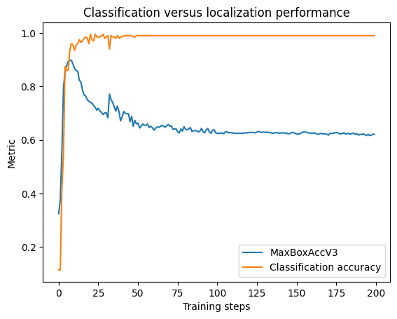
\includegraphics[width=0.7\textwidth]{fig_class_vs_localization.png}
    \caption[Classification versus localization accuracy]{Classification versus localization accuracy comparison of MinMaxCAM method for the VGG16-GAP model on the synthetic dataset.}
    \caption*{Source: Author}
    \label{fig:classification_versus_localization2}
    \end{center}
\end{figure}

During the early training epochs, both classification accuracy and localization accuracy improve. But in further epochs, classification accuracy keeps improving, while localization performance drops until they both converge.

The result shows that localization and classification performance may not necessarily correlate and further classification training may hurt localization performance. As classification accuracy improves, the model focuses on learning the most discriminative parts of an object to classify the image correctly. These discriminative parts only partially cover an object. As the localization objective is to cover the full object region, improving classification performance decreases localization accuracy. 

Therefore, it's important to use localization-only metrics like MaxBoxAccV3 and PxAP for model selection and evaluation of WSOL methods. To avoid learning a model which focuses on optimizing classification performance only, we stop the learning process when the validation loss hasn't decreased for five consecutive epochs.

\section{Computational complexity}
In this section we evaluation the computational complexity of \acrshort{cam} methods used in our experiments. We measure the localization method runtime for ResNet-50 network on the ImageNet validation dataset. The mean runtime and standard deviation per batch of images, and the aggregated runtime for the complete  dataset is computed. The results for each method is illustrated in Table \ref{tab:runtime_resnet50_imagenet}.

\begin{table}[ht]
\centering
\begin{tabular}{lrrrr}
\toprule
\multicolumn{2}{c}{} & \multicolumn{3}{c}{runtime (ms)} \\
method & batch size (bytes) & sum & mean & std \\
\cmidrule(lr){1-2} \cmidrule(lr){3-5}
CAM & 512 & 309209 & 3155 & 225 \\
Grad-CAM++ & 128 & 804349 & 2057 & 140 \\
MinMaxCAM & 512 & 299392 & 3055 & 982 \\
Score-CAM & 512 & \bfseries 97763413 & 997585 & 34463\\
\bottomrule
\end{tabular}
\caption[Method runtime for ResNet-50 on ImageNet validation dataset]{Method runtime for ResNet-50 on ImageNet validation dataset.}
\label{tab:runtime_resnet50_imagenet}
\end{table}

The runtime is measured as the time it takes to compute score maps for the 50000 images in the ImageNet validation dataset. Runtime exludes operations to load and preprocess the images. Grad-CAM was not measured as this method specializes to the CAM method for ResNet-50. However, it has the same order of complexity as Grad-CAM++ due to the equal number of forward and backward passes. Grad-CAM++ takes nearly three times the runtime of the CAM method. This could indicate that backward passes more costly than forward passes.

Each method computes a score map as a weighted combination of feature maps in the final convolutional layer. CAM (MinMaxCAM uses the CAM method for computing score maps), takes as weights the parameters learned in the single fully connected layer, which is a very cheap operation. Grad-CAM and Grad-CAM++ compute weights from the backprogagated gradients in the final convolutional layer. Similarly this operation is not computationally expensive.

The most computationally costly method by far is Score-CAM. This method computes the weights for the feature maps by feeding the network with the product of each feature map with the original image to obtain the classification score after softmax. As ResNet-50 has 2048 channels in its final convolutional layer, this is an expensive operation.

\section{Localization improvements}

Using the iterative localization method proposed in section \ref{sec:method_localization_improvement}, we analyze the effect of this method for VGG16-GAP and ResNet-50 architectures on the synthetic and ImageNet datasets. We use the same models that were trained for the non-iterative approach.

\subsection{Recall versus precision}
The aim of the iterative approach is to maximize the accurate localization of ground truth object instances. This is measured by the recall metric. If we would have a localization method that exhaustively generates bounding boxes of different granularity, then such method would accurately localize most object instances and thus have a high recall. At the same time this method would suffer from a lot of false positives, i.e., many localized objects would not match with the actual ground truth instances. Hence, the precision would be low.

To measure the impact of the iterative localization method we want to measure both precision and recall. Ideally, we would like to have a localization method that has good precision and recall. If we equally care about precision and recall, the f1 score represents the harmonic mean between precision and recall.

\subsection{Evaluation on synthetic datasets}
Here we evaluate the results of the iterative localization method for the VGG16-GAP network and the ResNet-50 network on the synthetic test datasets. We only tests the datasets that have images with a background to evaluate the effect of using different bounding box mask strategies.

\subsubsection{VGG16-GAP}

\begin{table}[ht]
\centering
\begin{tabular}{llrrrrrrrrr}
\toprule
     &       & \multicolumn{3}{c}{recall} & \multicolumn{3}{c}{precision} & \multicolumn{3}{c}{f1} \\
stop & merge & add & drop & unify & add & drop & unify & add & drop & unify \\
\cmidrule(rl){1-2} \cmidrule(rl){3-5} \cmidrule(rl){6-8} \cmidrule(rl){9-11}
\multirow[t]{3}{*}{0.25} & mean & 54.29 & 52.13 & 52.21 & \color{teal} \bfseries 54.09 & 61.21 & 61.30 & 54.19 & 56.30 & 56.39 \\
 & random & 53.92 & 52.04 & 51.75 & 53.26 & 62.28 & 62.06 & 53.59 & 56.70 & 56.44 \\
 & zero & \color{purple} \bfseries 52.92 & \color{purple} \bfseries 51.00 & \color{purple} \bfseries 50.96 & 53.20 & \color{teal} \bfseries 62.50 & \color{teal} \bfseries 62.31 & 53.06 & 56.17 & 56.07 \\
\multirow[t]{3}{*}{0.5} & mean & 56.75 & 54.29 & 55.71 & 52.41 & 59.86 & 61.02 & \color{teal} \bfseries 54.49 & 56.94 & \color{teal} \bfseries 58.24 \\
 & random & 56.88 & 54.08 & 54.54 & 52.25 & 61.45 & 61.99 & 54.46 & \color{teal} \bfseries 57.53 & 58.03 \\
 & zero & 54.42 & 52.12 & 52.38 & 52.11 & 61.15 & 61.33 & 53.24 & 56.28 & 56.50 \\
\multirow[t]{3}{*}{1.0} & mean & 64.25 & \color{teal} \bfseries 58.67 & 61.00 & 39.93 & 48.44 & 48.27 & 49.25 & 53.06 & 53.89 \\
 & random & \color{teal} \bfseries 64.50 & 58.17 & \color{teal} \bfseries 64.17 & 38.93 & \color{purple} \bfseries 46.63 & 52.33 & 48.55 & \color{purple} \bfseries 51.76 & 57.65 \\
 & zero & 62.83 & 58.08 & 59.17 & \color{purple} \bfseries 36.93 & 47.53 & \color{purple} \bfseries 45.97 & \color{purple} \bfseries 46.52 & 52.28 & \color{purple} \bfseries 51.74 \\
\bottomrule
\end{tabular}
\caption[Iterative CAM localization for VGG16-GAP on synthetic dataset]{Iterative CAM localization for VGG16-GAP on synthetic dataset.}
\label{tab:iter_metrics_vgg16_cam_synthetic}
\end{table}

\begin{table}[ht]
\centering
\begin{tabular}{lrrr}
\toprule
 & recall & precision & f1 \\
method &  &  &  \\
\cmidrule(lr){1-1} \cmidrule(lr){2-4}
CAM & \color{purple} \bfseries 55.71 & \color{purple} \bfseries 61.02 & \color{purple} \bfseries 58.24 \\
Grad-CAM++ & 55.75 & 61.24 & 58.37 \\
MinMaxCAM & 55.88 & 61.63 & 58.61 \\
Score-CAM & \color{teal} \bfseries 57.33 & \color{teal} \bfseries 62.90 & \color{teal} \bfseries 59.99 \\
\bottomrule
\end{tabular}
\caption[Iterative localization methods for VGG16-GAP on synthetic dataset]{Iterative localization methods for VGG16-GAP on synthetic dataset for mask=mean, merge=unify, stop=0.5.}
\label{tab:iter_metrics_vgg16_cam_synthetic_all}
\end{table}

\begin{figure}[ht]
    \begin{center}       
    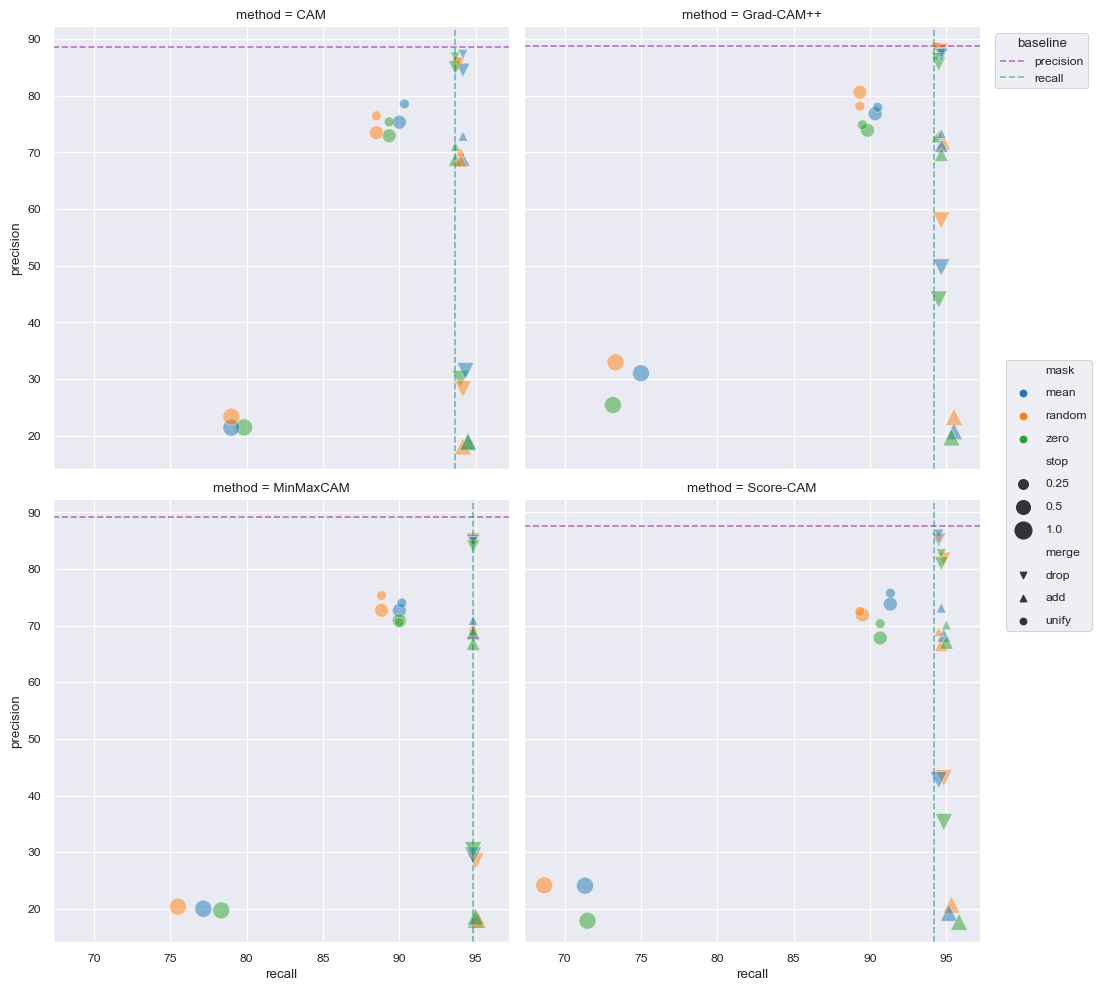
\includegraphics[width=1.0\textwidth]{images/fig_iter_vgg16_gap_syn_d1b.png}
    \caption[Iterative localization performance for VGG16-GAP on synthetic dataset d1b]{Iterative localization performance for VGG16-GAP on synthetic datasets d1b. The cross-hair lines mark the best precision and recall for non-iterative localization.}
    \caption*{Source: Author}
    \label{fig:prec_iter_vgg16_gap_syn_d1b}
    \end{center}
\end{figure}

\begin{figure}[ht]
    \begin{center}       
    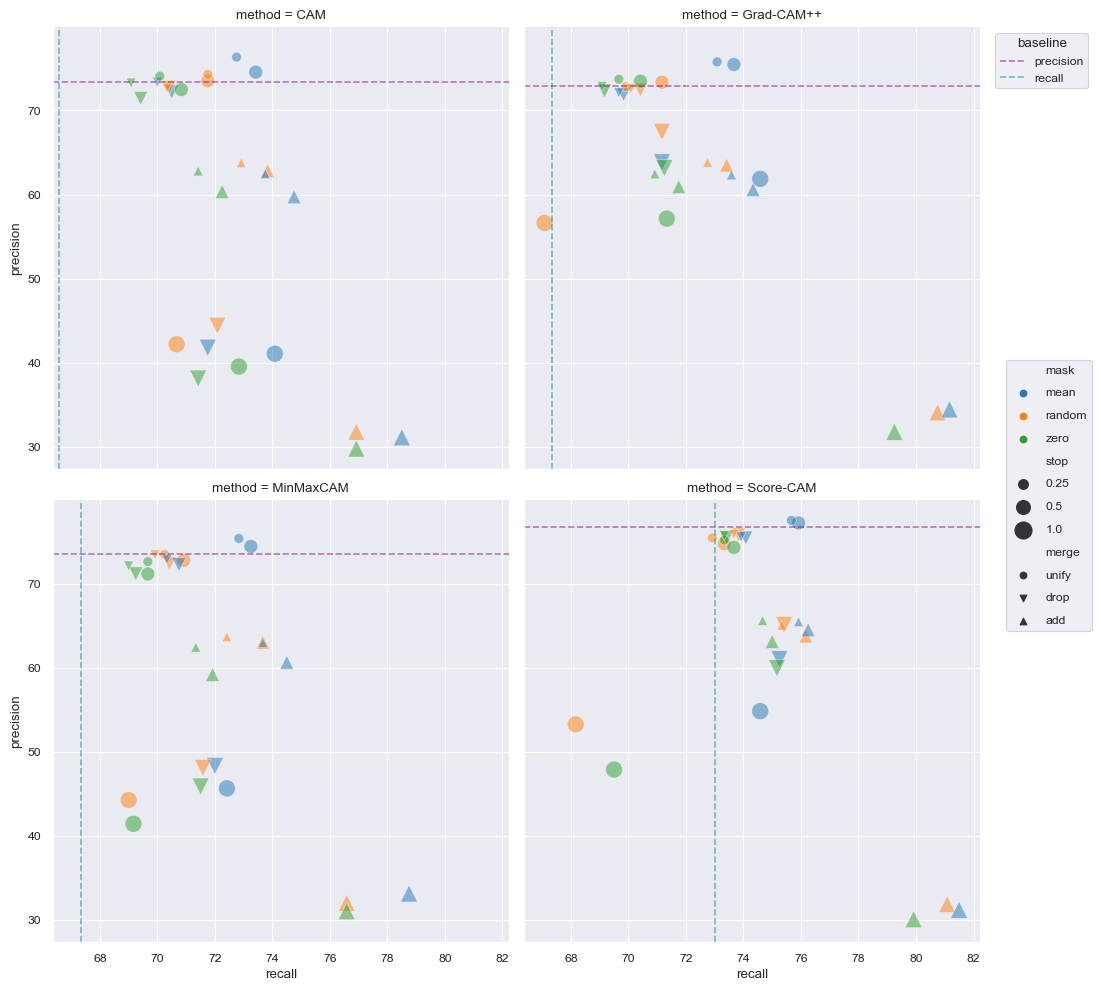
\includegraphics[width=1.0\textwidth]{images/fig_iter_vgg16_gap_syn_d2b.png}
    \caption[Iterative localization performance for VGG16-GAP on synthetic dataset d2b]{Iterative localization performance for VGG16-GAP on synthetic datasets d2b. The cross-hair lines mark the best precision and recall for non-iterative localization.}
    \caption*{Source: Author}
    \label{fig:prec_iter_vgg16_gap_syn_d2b}
    \end{center}
\end{figure}

\begin{figure}[ht]
    \begin{center}       
    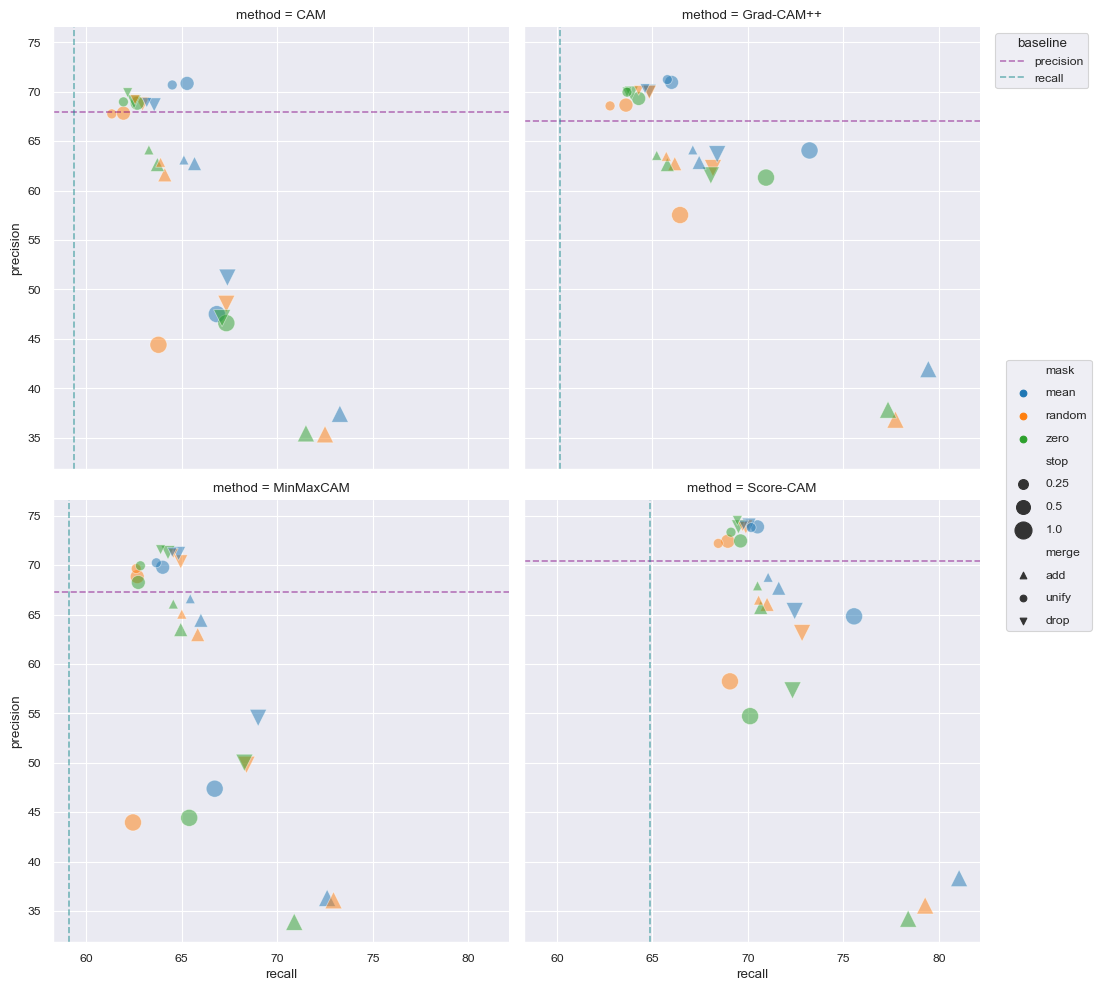
\includegraphics[width=1.0\textwidth]{images/fig_iter_vgg16_gap_syn_d3b.png}
    \caption[Iterative localization performance for VGG16-GAP on synthetic dataset d3b]{Iterative localization performance for VGG16-GAP on synthetic datasets d3b. The cross-hair lines mark the best precision and recall for non-iterative localization.}
    \caption*{Source: Author}
    \label{fig:prec_iter_vgg16_gap_syn_d3b}
    \end{center}
\end{figure}

\begin{figure}[ht]
    \begin{center}       
    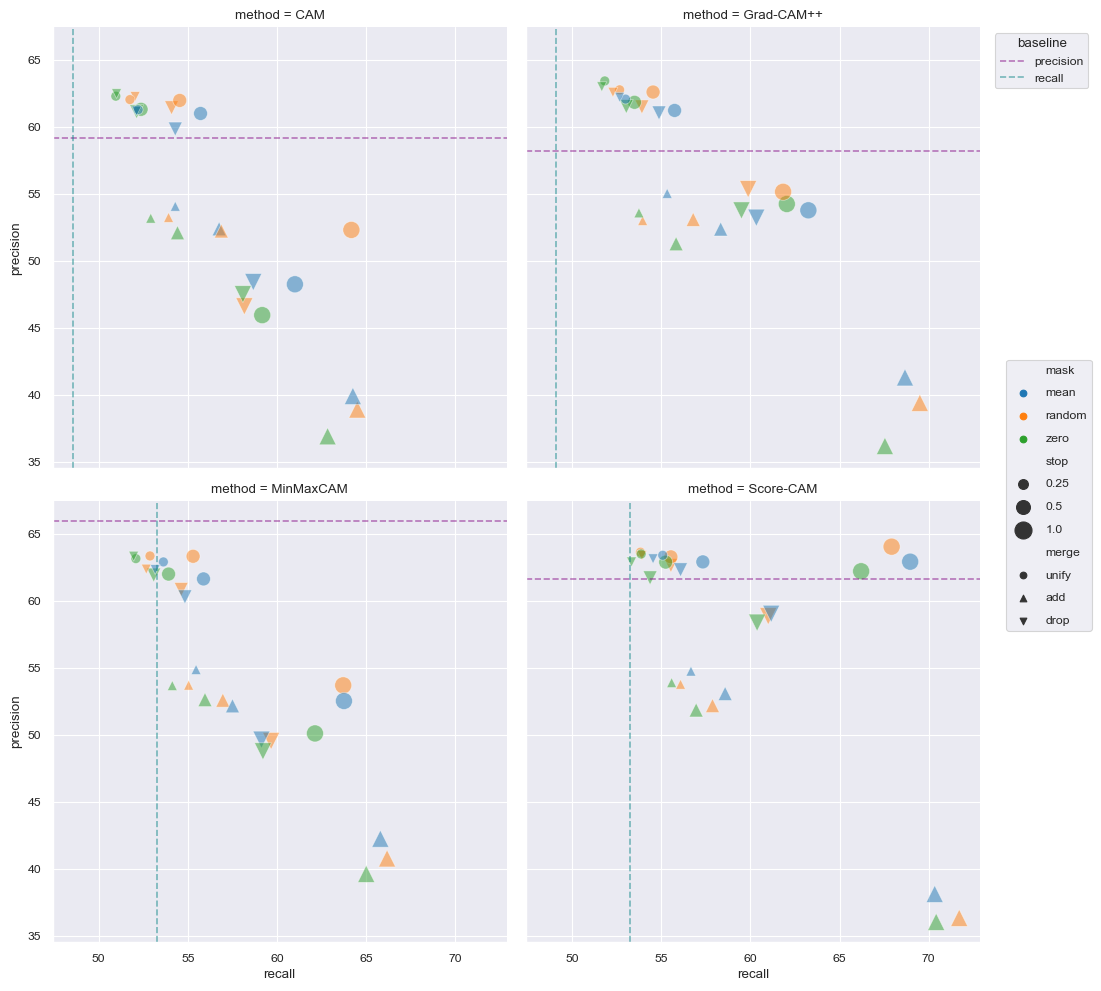
\includegraphics[width=1.0\textwidth]{images/fig_iter_vgg16_gap_syn_d4b.png}
    \caption[Iterative localization performance for VGG16-GAP on synthetic dataset d4b]{Iterative localization performance for VGG16-GAP on synthetic datasets d4b. The cross-hair lines mark the best precision and recall for non-iterative localization.}
    \caption*{Source: Author}
    \label{fig:prec_iter_vgg16_gap_syn_d4b}
    \end{center}
\end{figure}

\subsubsection{ResNet-50}

\subsection{Evaluation for ResNet-50 on ImageNet dataset}

\begin{figure}[ht]
    \begin{center}       
    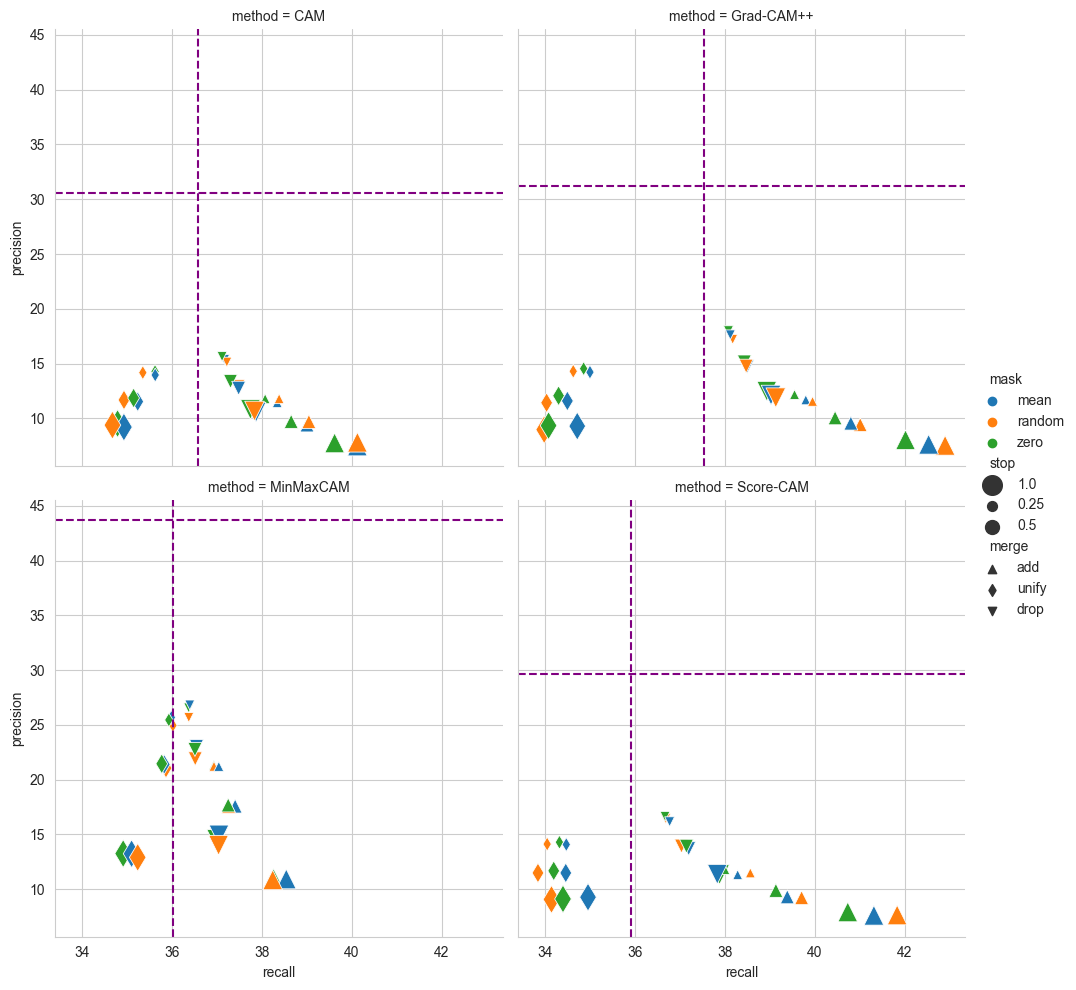
\includegraphics[width=1.0\textwidth]{fig_iter_resnet50_imagenet.png}
    \caption[Iterative localization performance for ResNet-50 on ImageNet dataset]{Iterative localization performance for ResNet-50 on ImageNet dataset. The cross-hair lines mark the best precision and recall for non-iterative localization.}
    \caption*{Source: Author}
    \label{fig:prec_iter_resnet50_imagenet}
    \end{center}
\end{figure}
